\subsubsection{\texttt{RF-4}: obtención bajo demanda de ficheros de ejercicios}
\label{subsec:rf4}

\begin{figure}[ht!]
    \centering
    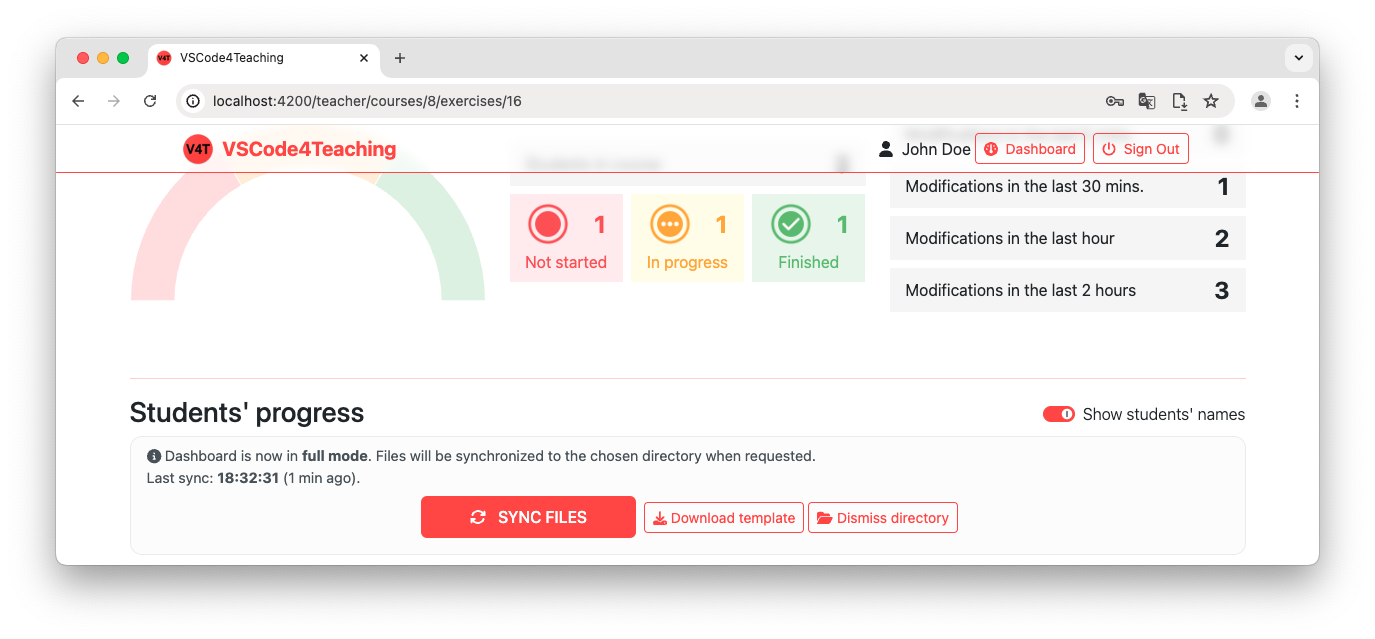
\includegraphics[width=\textwidth]{imagenes/utilizadas/4-3-implementacion/rf4-1.png}
    \caption{Fragmento del \textit{dashboard} que informa sobre la descarga de los ficheros de las propuestas de resolución de los estudiantes.}
    \label{fig:reqf4-1}
\end{figure}

El \textit{dashboard} de cada ejercicio disponible en la extensión permite, en su formato completo, abrir los ficheros que conforman la propuesta de resolución de cada estudiante y, además, visualizar gráficamente en Visual Studio Code las diferencias existentes entre las propuestas y la plantilla original. Análogamente, y dentro de las capacidades que permiten las tecnologías empleadas (descritas en la \referenciaSeccion{subsec:tecAppWeb}), la aplicación web brinda a los docentes la capacidad de descargar bajo demanda todas las propuestas de resolución para poder visualizarlas en local en el editor de su preferencia.

El requisito \referenciaConTT{subsec:rf3}{RF-3} introduce el funcionamiento y las capacidades de las que dispone el \textit{dashboard} de ejercicios implementado en la aplicación web. En la sección acerca del progreso de los estudiantes, tal como se puede apreciar en la \referenciaFigura{fig:reqf3-1}, se dispone un botón ``Choose directory'' (elegir directorio) que permite a los docentes escoger una carpeta en su máquina sobre la que concederán permisos de lectura y escritura para descargar en ella las propuestas de resolución de los estudiantes bajo demanda.

Tal como refleja la \referenciaFigura{fig:reqf4-1}, al escoger una carpeta local se habilitan nuevas opciones para los docentes, análogas al ``modo completo'' del \textit{dashboard} de la extensión, permitiendo la sincronización de los ficheros de los estudiantes bajo demanda, registrando cuándo fueron descargados por última vez. Esta sincronización es unidireccional, ya que no se registran las modificaciones locales realizadas por los docentes y, además, la descarga sobrescribe los ficheros previamente existentes en local. Se permite al profesor, adicionalmente, descargar la plantilla del ejercicio (y la propuesta de solución si la tuviera) en el mismo directorio.
